\section{Casos d'ús}\label{sec:analysis-visualization-use-cases}

Hem definit uns quants casos d'ús prou representatius que poden servir com a base:

\begin{itemize}
    \item Recurs més accedit durant un període de temps.
    \item Accessos amb el seu contingut alterat.
    \item Condicions d'accés dels accessos a recursos de l'EPSEVG.
\end{itemize}

\subsection{Recurs més accedit durant un període de temps}\label{subsec:most-accessed-resource}

\textbf{Definició}

\begin{itemize}
    \item Donat un període de temps, volem saber quin, o quins recursos són els més accedits.
    \item També volem esbrinar com ha sigut la seva evolució al llarg del temps, es tracta d'un pic puntual que altera les estadístiques, o s'ha mantingut constant?
    \item Quins paràmetres caracteritzen aquests accessos, vora quines hores es produeixen, mitjançant quins mètodes d'\gls{HTTP} es realitzen, quin és el codi de resposta més habitual, quin és el User Agent més comú\dots i molts més atributs.
\end{itemize}

\noindent \\
\textbf{Anàlisi}

\begin{itemize}
    \item Per esbrinar quins són els recursos més accedits, treballarem directament sobre la base de dades \textit{InfluxDB} .

    A causa de la gran quantitat de dades que s'han d'analitzar, \textit{Grafana} no podria ser capaç d'afrontar aquesta càrrega computacional.

    \item Per aquest període de temps, consultarem tots els accessos a recursos presents (que ja tenim marcats) i agregarem els seus identificadors.

    En acabar el procés, tindrem un conjunt d'identificadors cadascun amb el seu nombre d'aparicions.
    Ordenarem aquest conjunt i obtindrem els recursos més accedits.
\end{itemize}

\clearpage

\noindent \\
\textbf{Representació}

\begin{itemize}
    \item Per fer la representació de les dades primerament hem d'escollir una la tipologia de panells que volem utilitzar. Com estem parlant d'un anàlisi al llarg del temps, semblar que una sèrie temporal pot quadrar.

    \item Seleccionarem una gràfica de tipus \textit{Time Series} i afegirem a la part inferior la següent cerca.
    Concretament, estem cercant a \textit{InfluxDB}:
    \begin{itemize}
        \item Període del desembre del 2023.
        \item Accessos que siguin recursos i el seu \textit{\gls{handle}} (identificador) sigui \texttt{2099.1/18556}, que prèviament haurem determinat.
        \item Comptem cada accés i els agrupem per cada dia.
        \item La cerca que utilitzarem és la següent:
    \end{itemize}
\end{itemize}

\noindent
\begin{verbatim}
from(bucket: "upcommons")
  |> range(start: 2023-12-01T00:00:00Z, stop: 2023-12-31T23:59:59Z)
  |> filter(fn: (r) => r["_measurement"] == "tfg")
  |> filter(fn: (r) => r["_field"] == "recurs")
  |> filter(fn: (r) => r["_value"] == "2099.1/18556")
  |> aggregateWindow(every: 1d, fn: count, createEmpty: false)
  |> yield(name: "count")
\end{verbatim}

\clearpage

\noindent \\
\textbf{Resultat}

\begin{figure}[htbp]
    \centerline{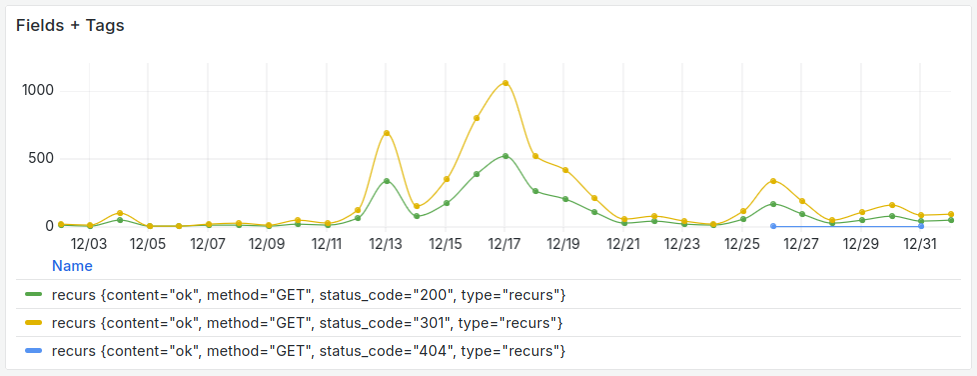
\includegraphics[width=\textwidth]{figures/most-accessed-resource}}
    \captionsetup{justification=centering}
    \caption[Representació del recurs més accedit durant el desembre del 2023.]{Representació del recurs més accedit durant el desembre del 2023. (\textbf{Font}: Elaboració pròpia.)}\label{fig:most-accessed-resource}
\end{figure}

\begin{itemize}
    \item Gràcies al fet que les entrades a la base de dades contenen els camps més rellevants, la classificació per cada paràmetre la realitza \textit{Grafana} automàticament.
    \item Com a conseqüència, per cada combinació del tipus de contingut (\textit{content}), mètode \gls{HTTP} emprat (\textit{method}) i resposta de la petició (\textit{status\_code}) que accedeixin a aquest recurs tindran el seu seguiment.
    \item Podem veure com sempre el contingut del registre d'accés és correcte (content = “ok”) i el mètode utilitzat és el GET.

    La resposta de la petició varia entre un \texttt{200} (succés) o un \texttt{301} (indica que el contingut és a una altra ubicació i et redirigeix)
\end{itemize}

\clearpage
\subsection{Accessos amb el seu contingut alterat}\label{subsec:content-altered-acces}

\textbf{Definició}

\begin{itemize}
    \item Donat un espai de temps, volem consultar quants accessos s'han produït amb malformacions al seu contingut.

    \begin{itemize}
        \item Les malformacions del contingut del accesos, tal i com vam veure a l'apartat de filtratge dels logs (vegeu~\ref{subsec:log-filter}), corresponen a registres que difereixen molt respecte el format general.
        \item Durant l'etapa d'anàlisi i emmagatzemmatge dels logs, vam marcar aquells sospitosos amb una etiqueta.
        Concretament, amb content = “diferent”.
    \end{itemize}

    \item També volem esbrinar com ha sigut la seva evolució al llarg del temps, a més dels paràmetres que s'utilitzen.
\end{itemize}

\noindent \\
\textbf{Anàlisi}

\begin{itemize}
    \item Treballarem sobre l'eina d'observabilitat Grafana, analitzant aquells accessos a recursos que tinguin alteracions en el seu contingut.
\end{itemize}

\noindent \\
\textbf{Representació}

\begin{itemize}
    \item Per fer la representació de les dades escollirem una sèrie temporal.
    \item Seleccionarem una gràfica de tipus Time Series i afegirem a la part inferior la següent cerca.
    Concretament, estem cercant a \textit{InfluxDB}:

    \begin{itemize}
        \item Període del 2023.
        \item Accessos que siguin recursos i el seu contingut sigui diferent.
        \item Comptem els accessos cada trenta dies.
        \item La cerca que utilitzarem és la següent:
    \end{itemize}
\end{itemize}

\noindent
\begin{verbatim}
from(bucket: "upcommons")
  |> range(start: 2023-01-01T00:00:00Z, stop: 2023-12-31T00:00:00Z)
  |> filter(fn: (r) => r["_measurement"] == "tfg")
  |> filter(fn: (r) => r["_field"] == "log")
  |> filter(fn: (r) => r["type"] == "recurs")
  |> filter(fn: (r) => r["content"] == "diferent")
  |> aggregateWindow(every: 30d, fn: count, createEmpty: false)
  |> yield(name: "count")
\end{verbatim}

\clearpage

\noindent \\
\textbf{Resultat}

\begin{figure}[htbp]
    \centerline{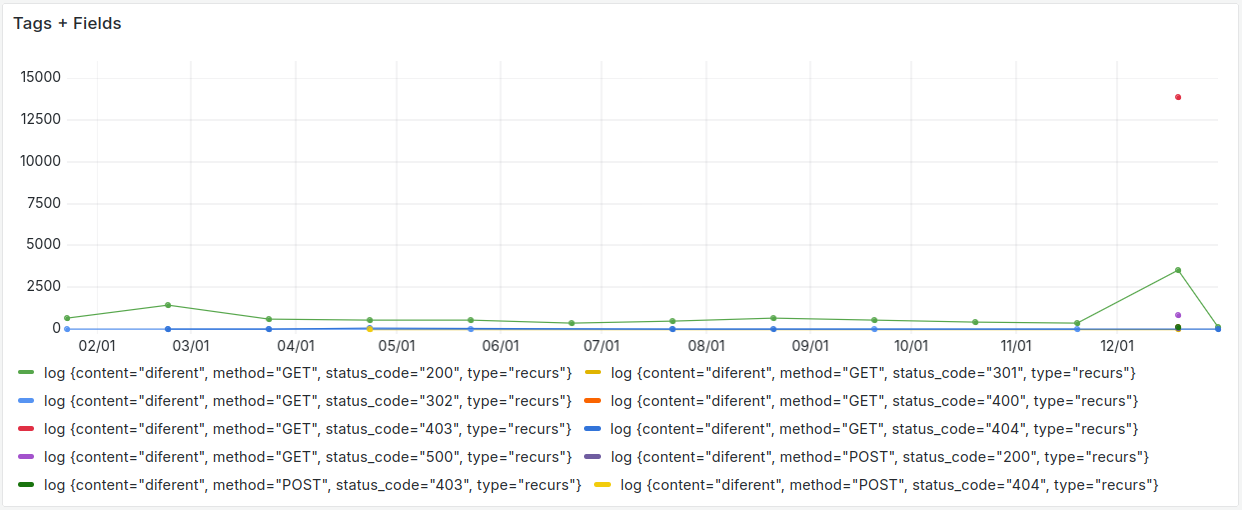
\includegraphics[width=\textwidth]{figures/possible-attacks}}
    \captionsetup{justification=centering}
    \caption[Representació del accessos amb el seu contingut alterat del 2023.]{Representació del accessos amb el seu contingut alterat del 2023. (\textbf{Font}: Elaboració pròpia.)}\label{fig:log-altered}
\end{figure}

\begin{itemize}
    \item Aquest seria el recompte d'accessos a recursos amb el contingut alterat durant l'any 2023, separats per mètode i codi d'estat.
    \item Vora finals d'any, podem observar com hi ha un pic de peticions que no és gens habitual.
    Concretament són peticions GET que retornen un 403.
    \item El codi d'estat 403 del protocol \gls{HTTP} que no estat autoritzat per realitzar aquesta petició.
    \item Explorant una mica més, obtenim que aquest pic correspon a una llarga sèrie de peticions que va augmentar considerablement a partir de les 10:30 h de l'11 de novembre del 2023 i hauria acabat quinze minuts després.
    \clearpage
    \begin{figure}[htbp]
        \centerline{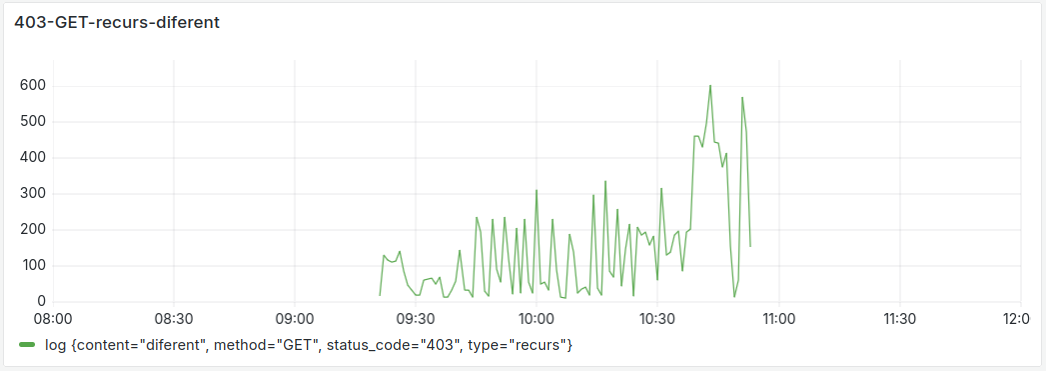
\includegraphics[width=\textwidth]{figures/possible-attacks-403}}
        \captionsetup{justification=centering}
        \caption[Pic de peticions del tipus \texttt{GET} que retornen un codi \texttt{403}.]{Pic de peticions del tipus \texttt{GET} que retornen un codi \texttt{403}. (\textbf{Font}: Elaboració pròpia.)}\label{fig:possible-attacks}
    \end{figure}
    \item Per consultar el contingut d'aquestes peticions ens redirigim a \textit{InfluxDB} i consultem les hores i els paràmetres prèviament determinats.
    \item El patró que segueix és consultar un recurs i afegir paràmetres d'\gls{HTTP} amb valors maliciosos.
    Els més habituals que s'han utilitzat són filter i range.
    La majoria d'aquests registres intenten executar un sleep.
    \item Un exemple, la comparació de dues comandes que retornen el mateix resultat sempre és certa (en vermell), i s'intenta executar un sleep per endarrerir la resposta certs segons. \\
    \begin{figure}[htbp]
        \centerline{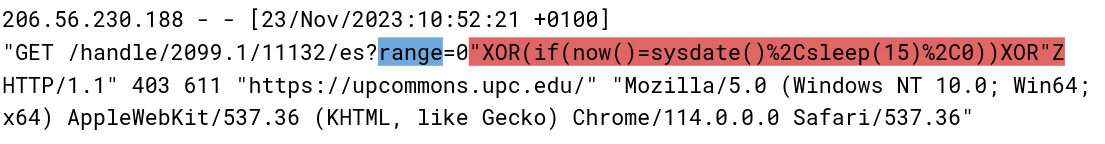
\includegraphics[width=\textwidth]{figures/log-attack}}
        \captionsetup{justification=centering}
        \caption[Exemple d'un intent d'atac a través d'un accés a un recurs.]{Exemple d'un intent d'atac a través d'un accés a un recurs. (\textbf{Font}: UPCommons.)}\label{fig:most-log-attack}
    \end{figure}
\end{itemize}

